\section{AVHRR infrared channel SRF comparison}
%==============================================
\label{app:srf}
The following are plots of the AVHRR/3 infrared SRF data from the \href{http://www.star.nesdis.noaa.gov/smcd/spb/fwu/solar_cal/spec_resp_func}{NESDIS/STAR website} (labeled as ``Official'') and those from the \href{ftp://monkey.ssec.wisc.edu/pub/srf}{CIMSS/SSEC ftp site} (labeled as ``HMW'') for the four AVHRR/3 instruments onboard NOAA-16, -17, -18, and MetOp-A. The interpolated SRFs are also shown as overplots. Apart from one set of instrument SRFs--that of the NOAA-17 AVHRR--at the scale that encompasses the entire SRF one cannot easily distinguish between the various SRFs.
\begin{figure}[htp]
  \centering
  \includegraphics[scale=1]{graphics/nominal/avhrr3_n16.srf.eps}
  \caption{Comparison of NOAA-16 AVHRR/3 Infrared channel SRFs.}
  \label{fig:avhrr3_n16}
\end{figure}

\begin{figure}[htp]
  \centering
  \includegraphics[scale=1]{graphics/nominal/avhrr3_n17.srf.eps}
  \caption{Comparison of NOAA-17 AVHRR/3 Infrared channel SRFs.}
  \label{fig:avhrr3_n17}
\end{figure}

\begin{figure}[htp]
  \centering
  \includegraphics[scale=1]{graphics/nominal/avhrr3_n18.srf.eps}
  \caption{Comparison of NOAA-18 AVHRR/3 Infrared channel SRFs.}
  \label{fig:avhrr3_n18}
\end{figure}

\begin{figure}[htp]
  \centering
  \includegraphics[scale=1]{graphics/nominal/avhrr3_metop-a.srf.eps}
  \caption{Comparison of MetOp-A AVHRR/3 Infrared channel SRFs.}
  \label{fig:avhrr3_metop-a}
\end{figure}

